% !TeX root = ../main.tex

\section{Methodology}
    \subsection{Observation Space}
    This study will use three cameras as input because intersection scenes require a wider field of view (FOV). 

    The target point is projected onto the vehicle's local coordinate system using a rotation matrix based on the current yaw angle:

    \begin{align*}
    lx &= dx \cdot \cos(-\psi) - dy \cdot \sin(-\psi) \\
    ly &= dx \cdot \sin(-\psi) - dy \cdot \cos(-\psi)
    \end{align*}

    \begin{table}[htbp]
    \centering
    \caption{Specification of Observation Components and Shapes.}
    \label{tab:observation_shapes}
    \begin{tabular}{lll}
    \toprule
    \textbf{Component} & \textbf{Shape} & \textbf{Range} \\
    \midrule
    Visual & $[4(\text{Frame}), \text{Height}, 3(n_{\text{camera}}) \times \text{Width}, 3(\text{RGB})]$ & $[0, 255]$ \\
    \addlinespace
    Goal   & $[2(\text{goal vector})]$ & $[-\infty, \infty]$ \\
    \bottomrule
    \end{tabular}
    \end{table}

    Here are some other parameters related to the camera:

    \begin{table}[htbp]
    \centering
    \caption{Camera Hyperparameters.}
    \label{tab:cam parameters}
    \begin{tabular}{ll}
    \toprule
    \textbf{Component} & \textbf{Value} \\
    \midrule
    Pixel & $[56\times56]$ \\
    \addlinespace
    FOV   & $60\degree$ \\
    \addlinespace
    Position & $[x=1.5,y=0,z=2]$ \\
    \bottomrule
    \end{tabular}
    \end{table}
    
    \subsection{Action Space}
    \cite{corrado_simulation-acquired_2022} pointed out that reinforcement learning requires a large number of interactions to converge in high-dimensional continuous control problems. By introducing a mapping mechanism to compress the high-dimensional action space into a low-dimensional latent action space, the data utilization efficiency and convergence speed of the agent can be directly improved. In this study, I simplified the three action spaces in \cite{elallid_improving_2024} into two action spaces: acceleration and steer.

    \begin{table}[htbp]
    \centering
    \caption{Specification of Action Components and Shapes.}
    \label{tab:action_shapes}
    \begin{tabular}{lll}
    \toprule
    \textbf{Component} & \textbf{Range} \\
    \midrule
    Steering & $[-1.0, 1.0]$ \\
    \addlinespace
    Acceleration/Brake  & $[-1.0, 1.0]$ \\    \bottomrule    
    \end{tabular}
    \end{table}

    \subsection{Reward feedback}
    The reward in this study is divided into three parts: 
    The global reward function $\mathcal{R}_{\text{total}}$ is structured hierarchically as formulated in Equation \ref{eq:total_reward}:
    \begin{equation}
        \mathcal{R}_{\text{total}} = \mathcal{R}_{\text{sparse}} + \mathcal{R}_{\text{shaping}} + \mathcal{R}_{\text{fine}}
        \label{eq:total_reward}
    \end{equation}
    \subsubsection{Sparse Reward}
    This reward is crucial to success or failure, directly determining the end of the round.

    When the agent safely reaches its destination, it receives a substantial termination sparse reward of $\mathcal{R}_{\text{success}} = +10.0$. Conversely, if the agent collides or leaves the road during the process, it will suffer a severe penalty of $\mathcal{R}_{\text{collision}} = \mathcal{R}_{\text{offroad}} = -10.0$.
    
    \subsubsection{Shaping Reward}
    To mitigate the typical vanishing policy gradient defect caused by purely sparse signals, the system introduces continuously shaping parameters to guide the model for efficient intersection crossing tracking.

    The distance reward $\mathcal{R}_d$ measures the decrease in physical Euclidean distance to the target between consecutive time steps $t-1$ and $t$. In the code execution of this study, this displacement value is first scaled down by a factor of 10 (multiplied by 0.1) to perform standard reward scaling, and then scaled up by a factor of 5 (multiplied by 5) to make the target more attractive to the agent, ultimately forming the form $\mathcal{R}_d = 0.5 \times (d_{t-1} - d_t)$. Meanwhile, the velocity reconstruction reward $\mathcal{R}_v$ undergoes bimodal optimization: to prevent the policy network from becoming overly conservative and stuck in place, any velocity below $0.5 \text{ m/s}$ triggers a dynamic penalty; for a compliant cruising speed profile, the policy is guided by a reward of $\min(v_t, 10.0) / 33.0$, capped at 10 m/s. This boundary setting is based on the evaluation results of \cite{elallid_improving_2024} on a right-turn baseline (this paper validates that the average tactical speed does not exceed $5 \text{ m/s}$ in complex intersection right-turn scenarios).
    
    \subsubsection{Fine Tune Reward}
    To prevent aberrant agent behavior such as sudden lane changes or illegal shortcuts, this study explicitly introduces micro-adjustment penalties as defined in the formula \ref{eq:total_reward}. Driving on or crossing a dashed line triggers a slight penalty of $\mathcal{R}_{\text{marking}} = -0.025$. Intruding into or driving in the oncoming lane represents a high risk and therefore triggers a severe risk-avoidance penalty of $\mathcal{R}_{\text{oncoming}} = -0.200$. This specific mathematical asymmetry (meaning the penalty for driving on the wrong side of the road is much greater than the penalty for crossing a dashed line) forces the policy gradient to strictly prioritize lane centering and adherence to standard traffic regulations, thereby ensuring vehicles navigate unsignaled intersections with elegant dynamic trajectories and compliant legal behavior.

    \subsection{Condition}
    The following are the triggering conditions for this study:

    \textbf{1) Collision Telemetry:} The collision signal is emitted by the collision sensor integrated in CARLA.

    \textbf{2) Oncoming Lane Invasion (Otherlane flag):} This study constructs a two-dimensional vector orientation alignment mechanism as shown in the formula \ref{eq:dot_product}. The simulation environment extracts the horizontal forward orientation vector $\mathbf{v}_{\text{ego}}$ of the main vehicle in real time and performs an algebraic dot product calculation with the legal driving direction vector $\mathbf{v}_{\text{lane}}$ mapped to the local lane heading point. When the scalar is positive (dot product > 0), it means the vehicle's direction is within the compliant envelope of $\pm 90^{\circ}$. Conversely, when the scalar is negative (dot product < 0), it indicates that the angle between the two vectors exceeds $90^{\circ}$, and the system will immediately trigger `otherlane flag` and activate the wrong-way penalty $\mathcal{R}_{\text{oncoming}}$.

    \textbf{3) Lane Marking Straddling (On marking flag):} When the spatial deviation between the vehicle's center coordinates and the lane centerline exceeds a critical threshold of approximately $1.40 \text{m}$, `on marking flag` will be triggered, identifying that the wheels have either touched or crossed the dashed line.

    \textbf{4) Roadway Departure (Off road flag):} When the sustained lateral deviation further increases to $\vert \Delta y \vert \ge 2.25 \text{ m}$, the system will determine that the vehicle has catastrophically left the road. Given that the physical width of the main body is approximately $2.0 \text{ m}$, a lateral offset of $2.25 \text{ m}$ mathematically means that more than $50\%$ of the vehicle's volume has crossed the solid road boundary, causing the vehicle to enter non-drivable areas such as grass, shoulders, or sidewalks.

    The directional alignment for oncoming lane invasion is mathematically formalized via the dot product of the vehicle's directional vectors:
    \begin{equation}
        \text{Invasion Trigger} = 
        \begin{cases} 
          \text{True (Otherlane\_flag)}, & \text{if } \mathbf{v}_{\text{ego}} \cdot \mathbf{v}_{\text{lane}} < 0 \\
          \text{False}, & \text{if } \mathbf{v}_{\text{ego}} \cdot \mathbf{v}_{\text{lane}} \ge 0
       \end{cases}
       \label{eq:dot_product}
    \end{equation}
    where $\mathbf{v}_{\text{ego}} = [x_{\text{ego}}, y_{\text{ego}}]^T$ and $\mathbf{v}_{\text{lane}} = [x_{\text{lane}}, y_{\text{lane}}]^T$ represent the localized 2D horizontal components of the ego vehicle's forward heading vector and the regulatory lane waypoint direction vector, respectively.
    
    Concurrently, the tracking boundary deviations $\Delta y$ from the idealized lane centerline dictate the micro-behavioral and structural failure states:
    \begin{equation}
        \text{State Status} = 
        \begin{cases} 
          \text{On\_marking\_flag}, & \text{if } 1.40 \text{ m} \le \vert \Delta y \vert < 2.25 \text{ m} \\
          \text{Off\_road\_flag}, & \text{if } \vert \Delta y \vert \ge 2.25 \text{ m}
       \end{cases}
    \end{equation}
    
    \subsection{Model Architecture}
    \subsubsection{Vision Transformer}
    \begin{figure}[t]
        \centering
        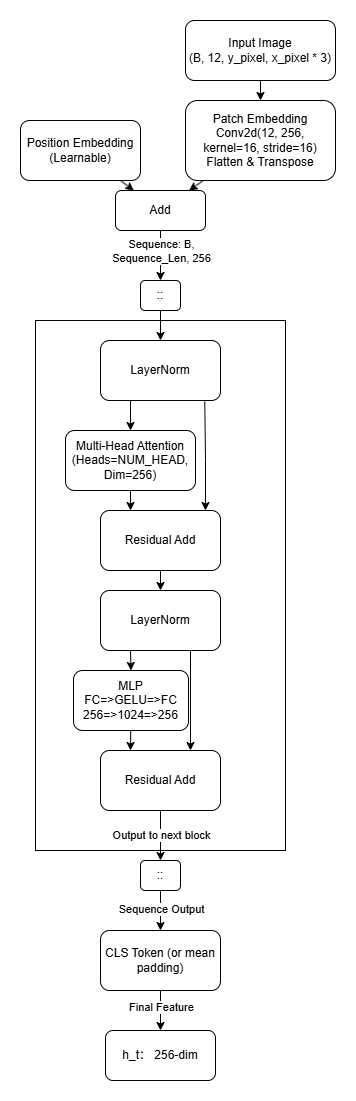
\includegraphics[width=0.3\textwidth]{figures/vit.png}
        \caption{The architectural visualization of Vision Transformer.}
        \label{fig:Vision Transformer Model}
    \end{figure}
    
    \ref{fig:Vision Transformer Model} show the architecture of the Vision Transformer network. The input shape of the ViT model in this study is $(B, 12, y_{pixels}, x_{pixels}\times3)$. $B$ is the batch size, and $12$ represents $3$ (RGB) × $4$ (frames). On the left is a learnable position embedding that adds positional information to each image patch. This helps the model identify the top-left and bottom-right image patches \cite{elallid_improving_2024}. The internal structure of the Transformer consists of 2 blocks and 8 heads. Finally, the output of ViT is a vector representing the "semantics of the entire image". This study uses the first label as the output. The final output is a 256-dimensional embedding feature vector. This vector will be used as state input for SAC (Soft Actor-Critic) algorithm to determine whether to "accelerate" or "brake".
    
    \subsubsection{Actor}
    \begin{figure}[t]
        \centering
        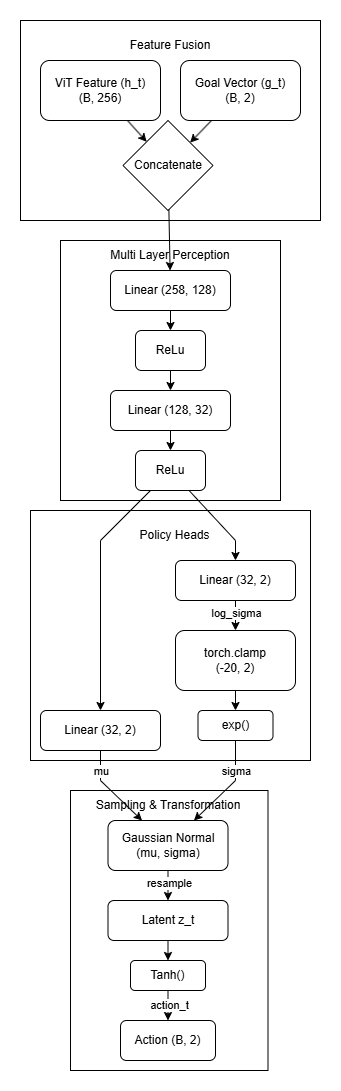
\includegraphics[width=0.3\textwidth]{figures/actor.png}
        \caption{The architectural visualization of Actor.}
        \label{fig:Actor architecture}
    \end{figure}
    \ref{fig:Actor architecture} show the architecture of the Actor. It combines the vector features output by ViT with the target vector and compresses it from 258 dimensions to 128 dimensions, and then further to 32 dimensions. The goal of this stage is to extract core signals from the fused features sufficient to determine driving behavior. Next comes probabilistic distribution modeling (policy head). The network branches here, outputting two parameters of a Gaussian distribution: mean ($\mu$): representing the ideal action center perceived by the model; standard deviation ($\sigma$): representing uncertainty or exploratory tendency in decision-making.
    
    \subsubsection{Double Critic}
    \begin{figure}[t]
        \centering
        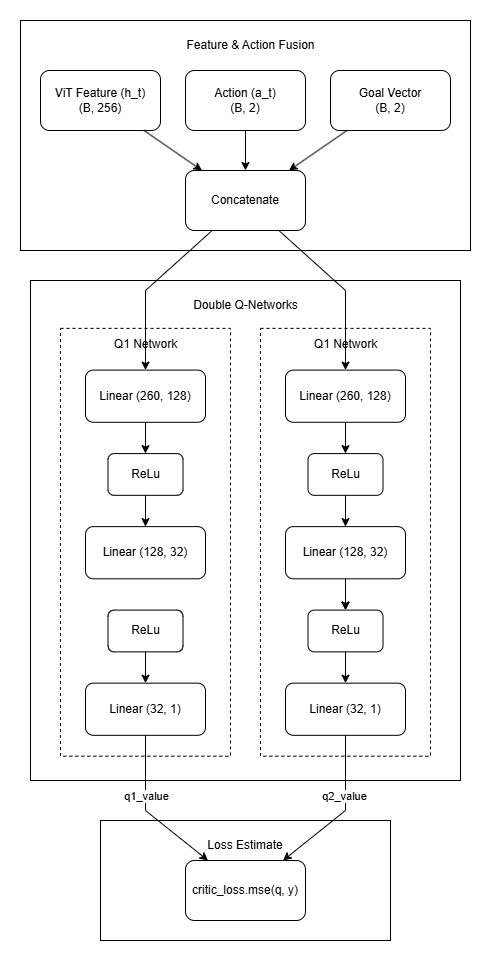
\includegraphics[width=0.3\textwidth]{figures/double critic.png}
        \caption{The architectural visualization of Critic.}
        \label{fig:Double Critic}
    \end{figure}
    \ref{fig:Double Critic} is a structure consisting of two evaluation networks. The first step is to concatenate the feature vector from the ViT output, target vector, and action, and then input the concatenated result into the two evaluation networks. Each channel in the evaluation network contains two fully connected layers (linear 260 $\pm$ 128 $\pm$ 32) with ReLU nonlinear activation. Finally, the error between the two evaluator outputs is calculated as a mean squared error (MSE) function, the results are summed, and then the network is updated.
    
    \subsubsection{Overview}
    \begin{figure}[t]
        \centering
        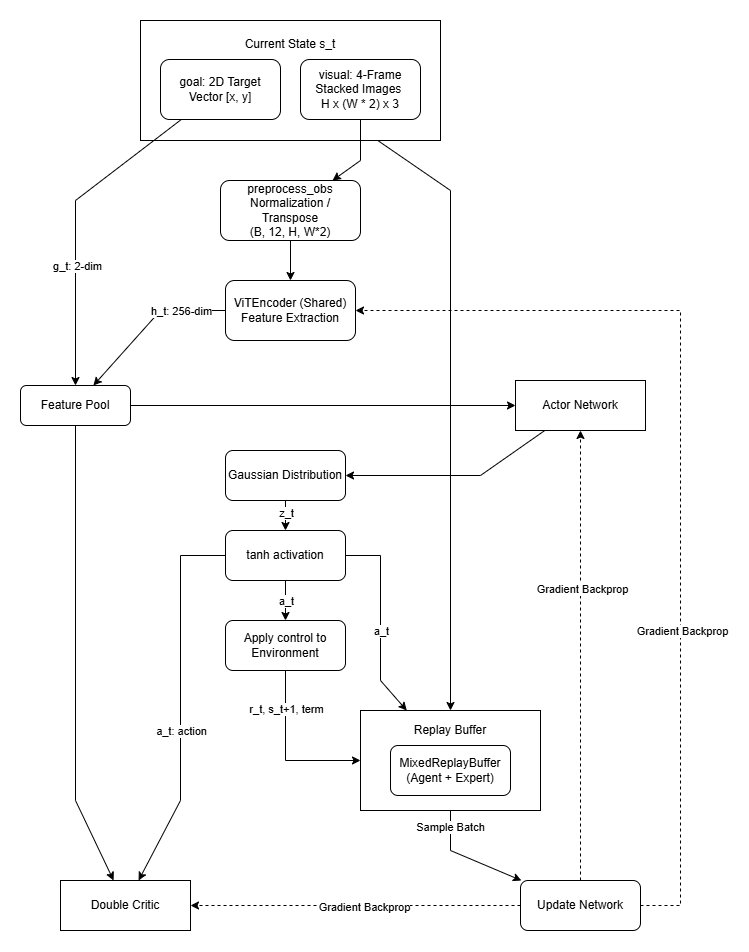
\includegraphics[width=0.3\textwidth]{figures/overview.png}
        \caption{Overview of the Model}
        \label{fig:Overview}
    \end{figure}
    \ref{fig:Overview} is the training workflow of the proposed ViT-SAC framework in this study.

    Perceptual Instantiation and Latent Space Encoding: Initially, the CARLA simulation environment instantiates the original state-space observation vector $\mathcal{S}_t$, which encapsulates the target vector and the original multi-camera, multi-frame visual pixel stream. The visual tensor undergoes normalization and resizing before being injected into the Vision Transformer (ViT) spatial encoder. ViT maps the high-dimensional visual input to a $256$-dimensional latent visual feature vector, which is temporarily archived in the structured feature library of the policy network.

    Random Action Generation and Boundary Constraints: Given that traffic light-free intersection navigation represents a highly complex task, the random actor network does not directly generate actions (steer and acceleration). Instead, the output of the policy head is a mean vector $\mu_t$ and a log-standard deviation vector $\log\sigma_t$ that can represent a Gaussian probability distribution. The system samples a potential action vector $z_t \sim \mathcal{N}(\mu_t, \sigma_t^2)$ based on a Gaussian probability distribution. The action vector is: $a_t = \tanh(z_t) \in [-1.0, 1.0]^2$. The two-dimensional output here represents the lateral steering torque and the longitudinal acceleration/braking command.

    Environmental Interaction: By executing $a_t$, the autonomous vehicle will interact with the CARLA environmental intersection and receive corresponding feedback (rewards or penalties). For example, a severe termination safety penalty of $-10.0$ is backpropagated when an adversarial collision telemetry signal is triggered.

    Asynchronous Experience Archive: The collected individual transition tuples—including the historical state $\mathcal{S}_t$, action $a_t$, environmental feedback (reward and penalty) $\mathcal{R}_{\text{total}}$, next state $\mathcal{S}_{t+1}$, and episode termination flag—are appended to \texttt{MixedReplayBuffer}. During concurrent training, the system samples mini-batch samples from this buffer to train and update the dual Critic network and Actor policy network. This single-step interaction pipeline is repeated over millions of temporal environmental steps.
    
    \subsubsection{Hyperparameter}
    \begin{table}[htbp]
    \centering
    \caption{The hyperparameters of this study}
    \label{tab:hyperparameter}
    \begin{tabular}{llc}
    \toprule
    \textbf{Notation} & \textbf{Meaning} & \textbf{Value} \\ \midrule
    $v_{max}$ & Velocity upper limit & 10 \\
    $v_{min}$ & Velocity lower limit & 0.5 \\
    $\gamma$ & Discount rate & 0.99 \\
    $N_{buffer}$ & Agent buffer capacity & 200000 \\
    $N_{A}$ & Agent buffer mini-batch size & 32 \\ 
    $N_{E}$ & Expert buffer mini-batch size & 32 \\ 
    $N_{BC}$ & Behavior clone batch size & 32 \\ 
    $T_{BC}$ & Iteration for Behavior clone & 100 \\ 
    $Block$ & Number of ViT blocks & 2 \\ 
    $Head$ & Number of ViT heads & 8 \\ 
    $N_{steps}$ & Training step & 500 \\ 
    $N_{patches}$ & Patches size & $14\times14$ \\ 
    $lr$ & Learning rate for critic and actor & 0.0003 \\ 
    $FPS$ & Frame per second & 5 \\ 
    \bottomrule
    \end{tabular}
    \end{table}

    The vast majority of the fundamental neural network architecture and reinforcement learning hyperparameters in this study inherit the structural configuration established by \cite{elallid_improving_2024}. These parameters include the empirical replay buffer capacity ($N_{\text{buffer}}$), the state encoder feature tracking exponent ($N_A, N_E$), the Vision Transformer configuration matrix including the encoded blocks ($B_{\text{lock}}$), the attention multi-head ($H_{\text{ead}}$), and the image patch segmentation density ($N_{\text{patches}}$), as well as the optimization learning rate ($lr$) and simulation frame rate ($FPS$).

    However, to exceed the boundary constraints defined in the referenced text, this study modifies the velocity envelope constraint based on exploratory empirical feedback: Velocity cap optimization ($V_{\max}$): Drawing on \cite{elallid_improving_2024} demonstration that the average speed limit for autonomous vehicles at roundabouts and unsignaled intersections does not exceed $5.0 \text{ m/s}$, this study strategically adjusts the maximum speed constraint $V_{\max}$ to $10.0 \text{ m/s}$. This improvement prevents the Soft Actor-Critic (SAC) agent from spending excessive training steps exploring drivable high-speed states, thereby accelerating policy convergence.

    Metastable idling penalty mechanism ($V_{\min}$): In the initial training phase, experiments observed that the policy network is highly susceptible to getting trapped in local optima. Specifically, frequent collisions or leaving the road in the early stages accumulate significant negative rewards, causing most episode scores to be below zero. To circumvent these penalties, stochastic policies degenerate into an "idle defense" mechanism, where vehicles choose to remain permanently stationary, exploiting loopholes by performing zero-speed actions to claim zero-step reward boundaries. To break this policy stagnation, this study introduces a deterministic stopping penalty mechanism indexed by a minimum speed threshold $V_{\min}$ into the reward, successfully leveraging a continuous gradient flow to drive the agent out of non-asymptotic local dead zones.